\chapter{Related Works}
\label{chap:related_works}

Research relevant to graph generation spans probabilistic graph modeling, graphon estimation, neural graph generation, diffusion models, graphon-based representations, and distributional evaluation. The theoretical foundations concerning graph representations, graph-generation challenges, graphons, and graphon estimation were introduced in Chapter~\ref{chap:background}. This chapter instead examines how representative methods from the literature instantiate these concepts computationally.

The discussion is organized according to the representation in which estimation or generation is performed, with particular attention to implicit graphon estimation, discrete diffusion, direct graph diffusion, graphon-mediated generation, and the evaluation of generated graph distributions.


\section{Probabilistic Graph Models}
\label{sec:probabilistic_graph_models}

Classical probabilistic graph models define graph distributions through explicit structural assumptions rather than learning unrestricted distributions from data. They remain useful reference models because they isolate properties such as homogeneous connectivity, community structure, degree heterogeneity, preferential attachment, and local clustering.


\subsection{Erd\H{o}s--R\'enyi model}
\label{subsec:erdos_renyi}

The independent-edge \(G(n,p)\) model, commonly included in the Erd\H{o}s--R\'enyi family and introduced in this form by Gilbert \cite{gilbert1959random}, was already presented through its constant-graphon representation in Section~\ref{subsec:constant_graphons}. Its defining assumption is that every unordered pair of distinct nodes is connected independently with the same probability \(p\).
The model therefore provides a reference case in which connectivity is homogeneous and no community, degree-specific, or local structural mechanism is imposed.
\begin{figure}[H]
    \centering
    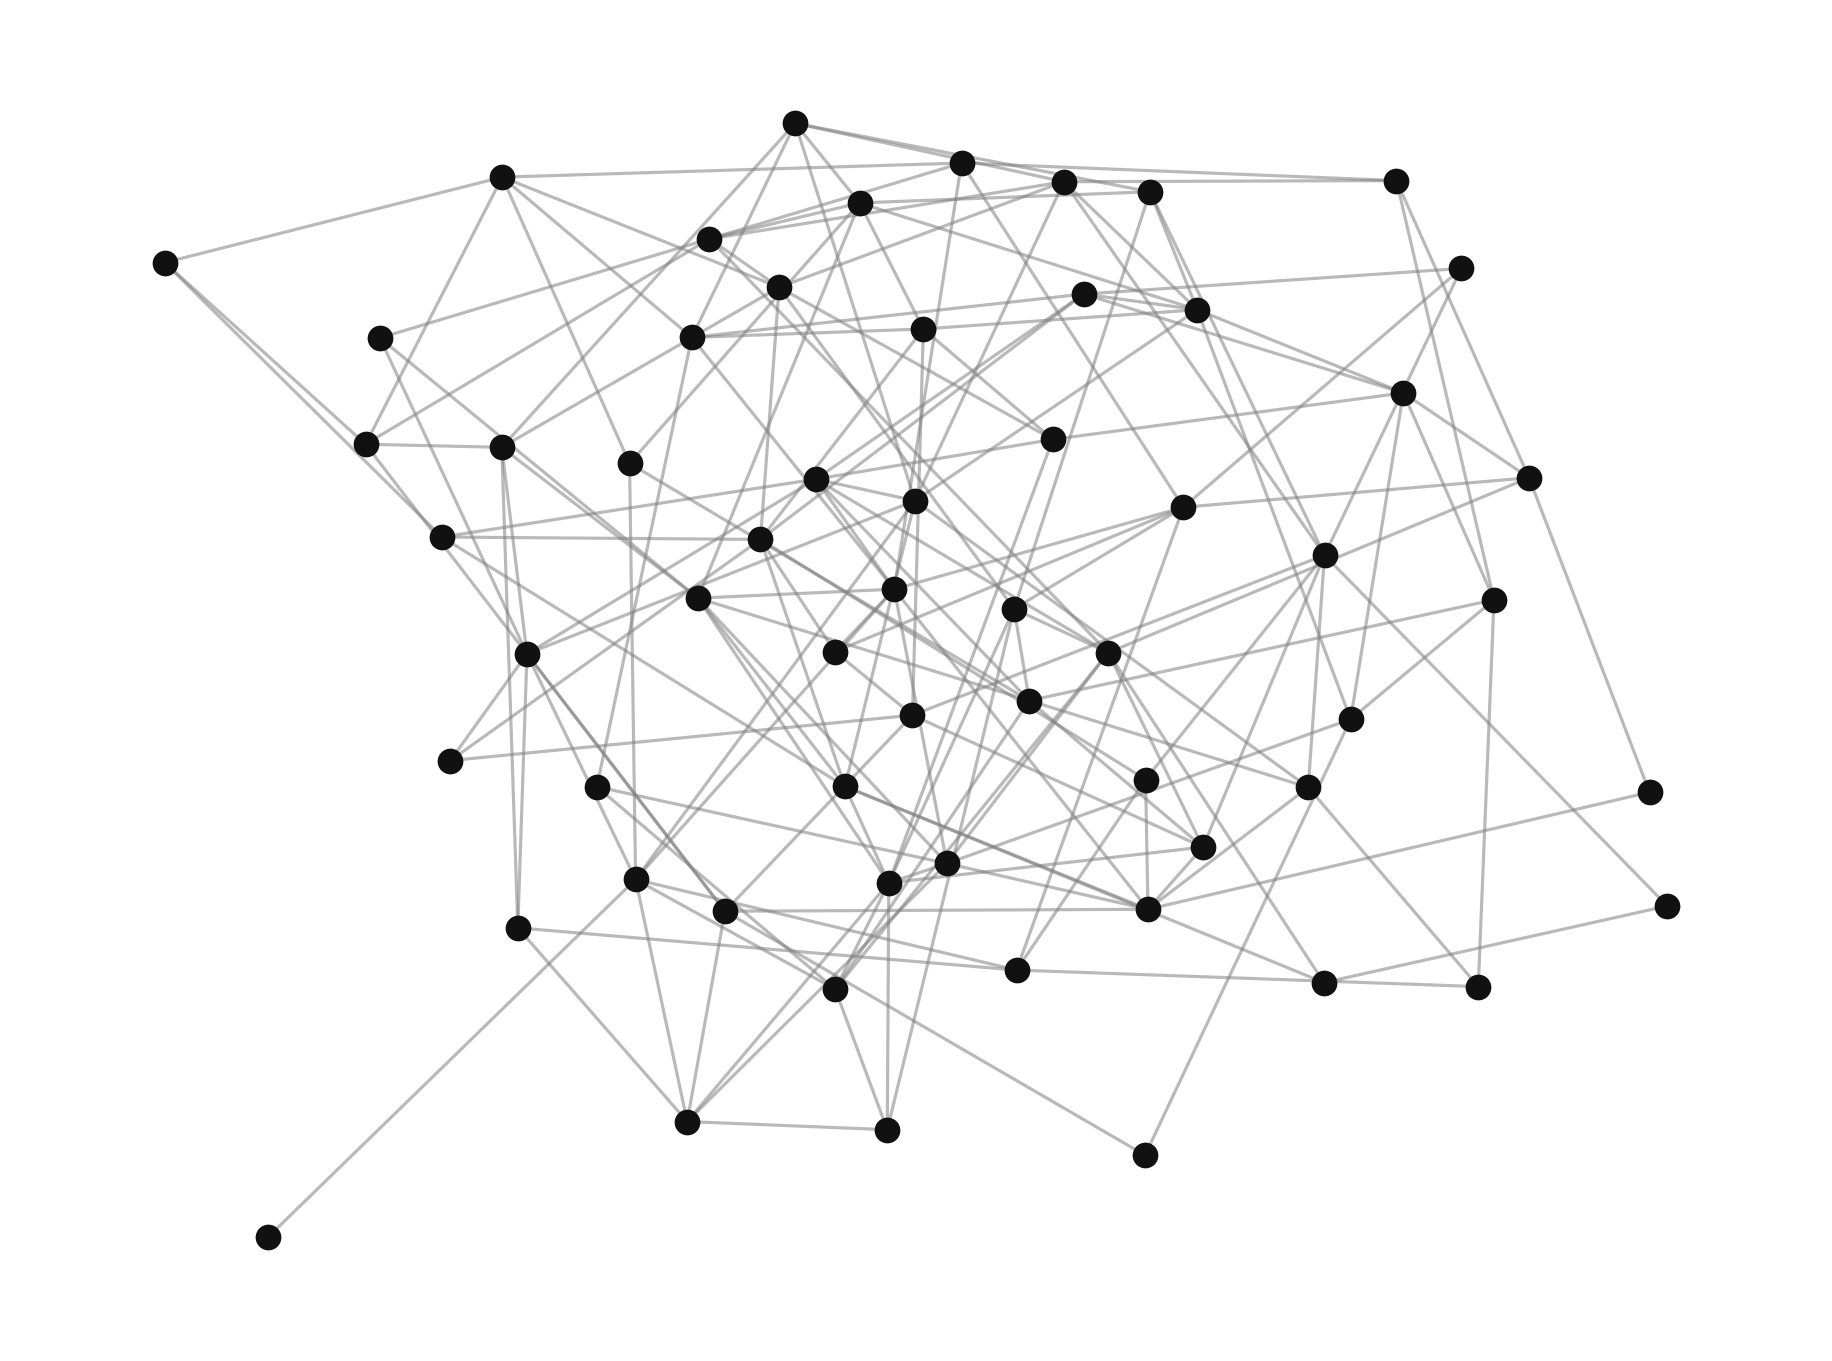
\includegraphics[width=0.5\textwidth]{figures/graph_models/erdos_renyi.png}
    \caption{Illustrative realization of an Erdős--Rényi graph with
    $n=60$ and edge probability $p=0.10$. Each pair of nodes is connected
    independently with the same probability, resulting in homogeneous
    random connectivity without an explicit community or hub structure.}
    \label{fig:erdos_renyi}
\end{figure}

\subsection{Stochastic Block Model}
\label{subsec:sbm}

The Stochastic Block Model (SBM) and its block-structured graphon representation were introduced in Section~\ref{subsec:block_graphons}. In the SBM, node connectivity is governed by latent block membership and a matrix of block-to-block connection probabilities \cite{holland1983stochastic}.

The model introduces community-level heterogeneity while retaining conditional independence of edges given the block assignments.
\begin{figure}[H]
    \centering
    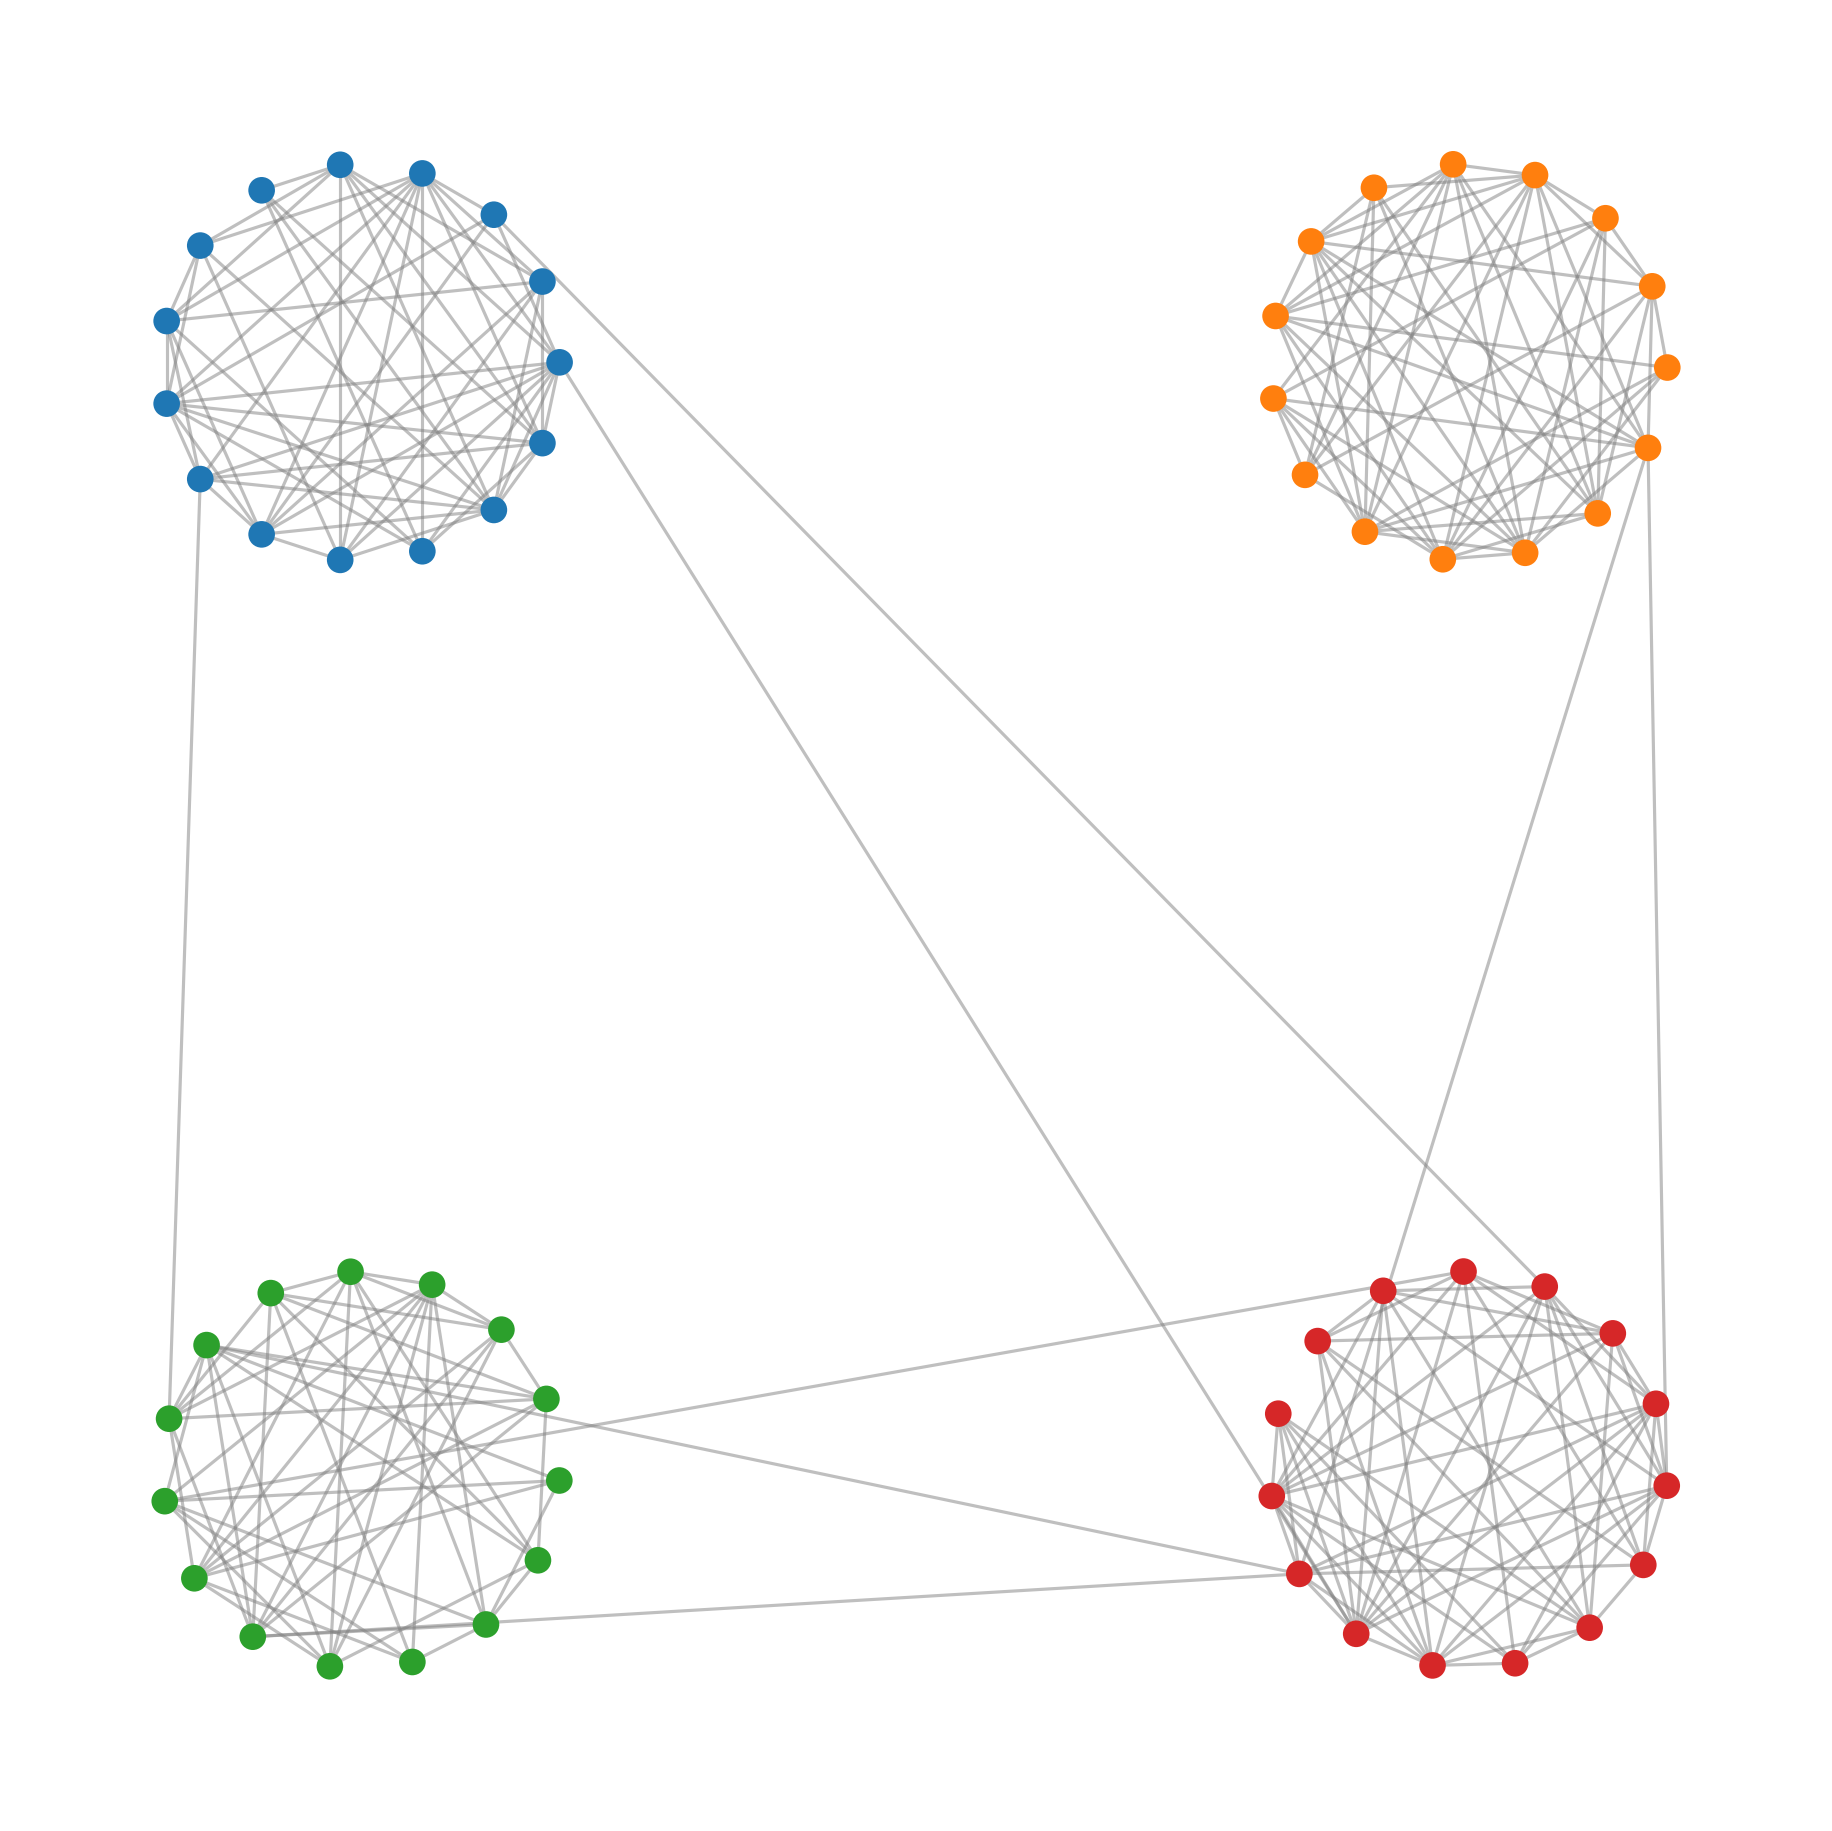
\includegraphics[width=0.4\textwidth]{figures/graph_models/stochastic_block_model.png}
    \caption{Illustrative realization of a Stochastic Block Model with four equally sized communities of 15 nodes. Edges are sampled with probability
    $p_{\mathrm{in}}=0.55$ within communities and $p_{\mathrm{out}}=0.006$ between communities. Node colors indicate block membership, 
    highlighting dense intra-community connectivity and sparse inter-community connections.}
    \label{fig:stochastic_block_model}
\end{figure}

\subsection{Degree-Corrected Stochastic Block Model}
\label{subsec:dcsbm}

The standard SBM cannot independently model substantial degree heterogeneity among nodes assigned to the same block. Karrer and Newman address this limitation through node-specific parameters \(\theta_i\) \cite{karrer2011stochastic}.

In their original formulation, the Degree-Corrected Stochastic Block Model is a Poisson multigraph model. For distinct nodes \(i\) and \(j\),

\[
A_{ij}
\sim
\operatorname{Poisson}
\left(
\theta_i\theta_j\omega_{z_i z_j}
\right),
\]

and therefore

\[
\mathbb{E}[A_{ij}]
=
\theta_i\theta_j\omega_{z_i z_j}.
\]

Here, \(z_i\) and \(z_j\) denote the block assignments, \(\omega_{z_i z_j}\) controls block-level interaction intensity, and \(\theta_i,\theta_j\geq0\) control node-specific degree propensities. Suitable normalization constraints are required for identifiability. The original model allows multiedges and self-edges, whereas simple-graph variants impose additional restrictions.
\begin{figure}[h!]
    \centering
    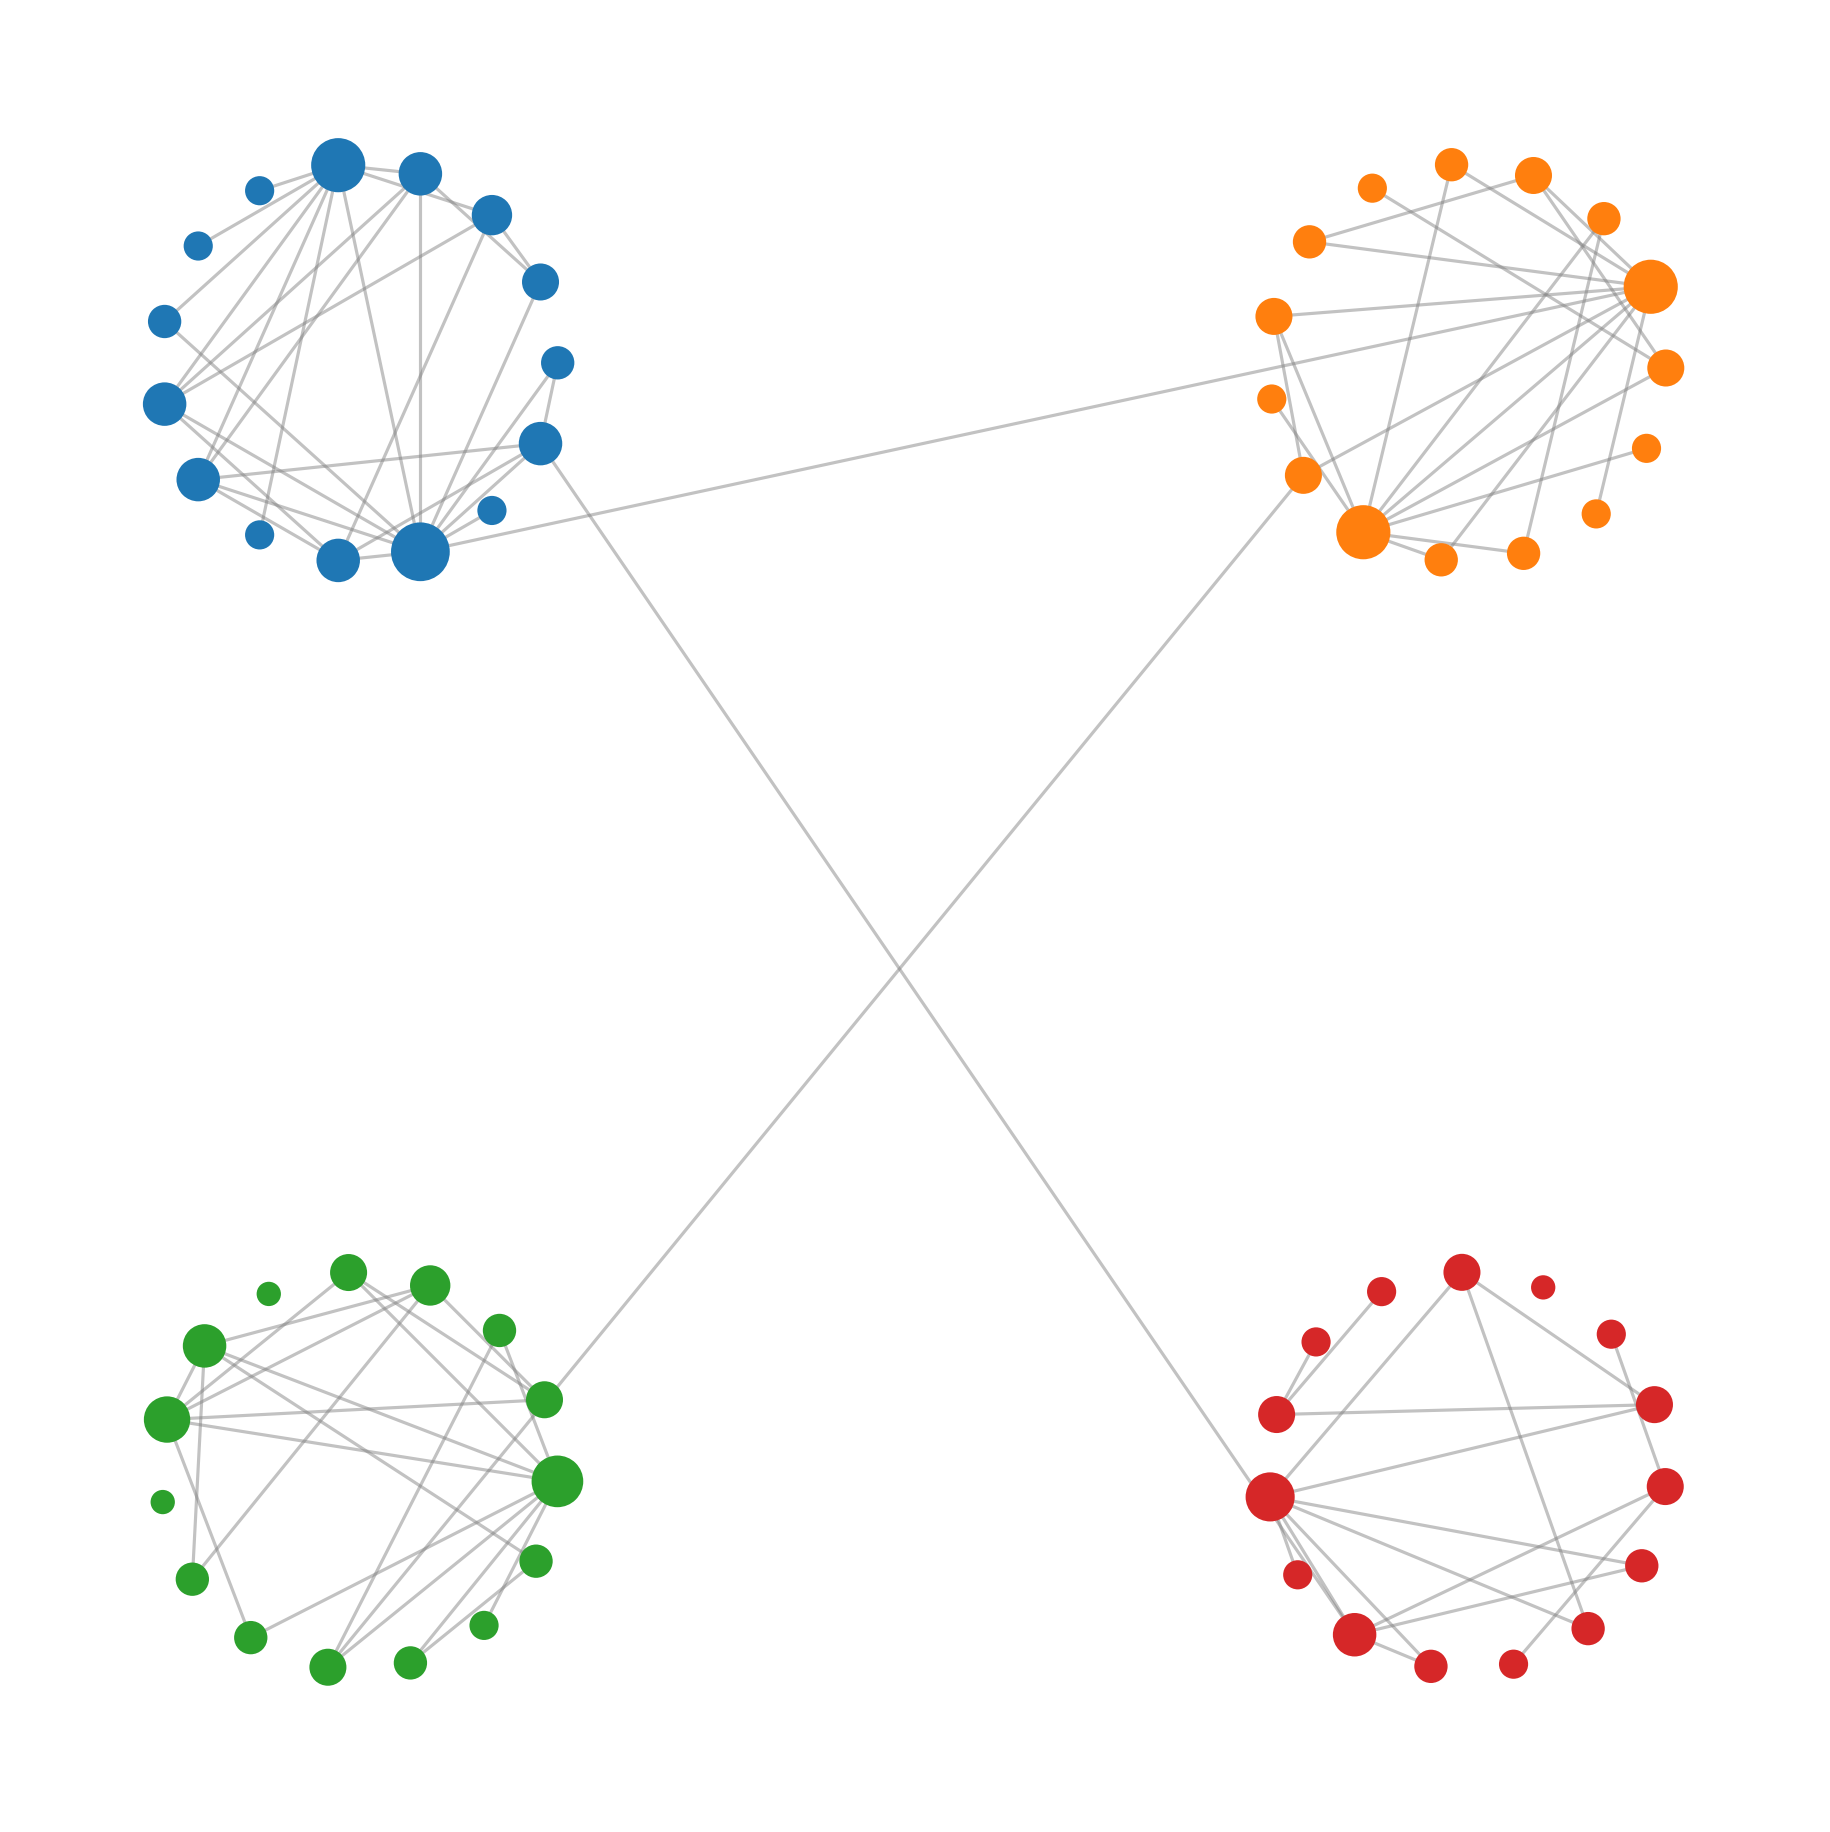
\includegraphics[width=0.5\textwidth]{figures/graph_models/degree_corrected_sbm.png}
    \caption{Illustrative realization of a Degree-Corrected Stochastic Block
    Model with four communities. Node colors indicate block membership, while
    heterogeneous node-specific degree propensities introduce substantial
    variation in connectivity within each community. Node size is proportional
    to the realized degree, emphasizing the within-block degree heterogeneity
    introduced by degree correction.}
    \label{fig:degree_corrected_sbm}
\end{figure}


\subsection{Configuration Model}
\label{subsec:configuration_model}

The Configuration Model generates random graphs from a prescribed degree sequence. Given degrees \(d_1,\ldots,d_n\), node \(i\) receives \(d_i\) half-edges, or stubs, which are paired to form edges. Depending on the chosen sample space, self-loops and multiple edges may occur; simple-graph variants impose additional restrictions \cite{fosdick2018configuring}.

The model preserves degree information while largely randomizing higher-order organization.
\begin{figure}[H]
    \centering
    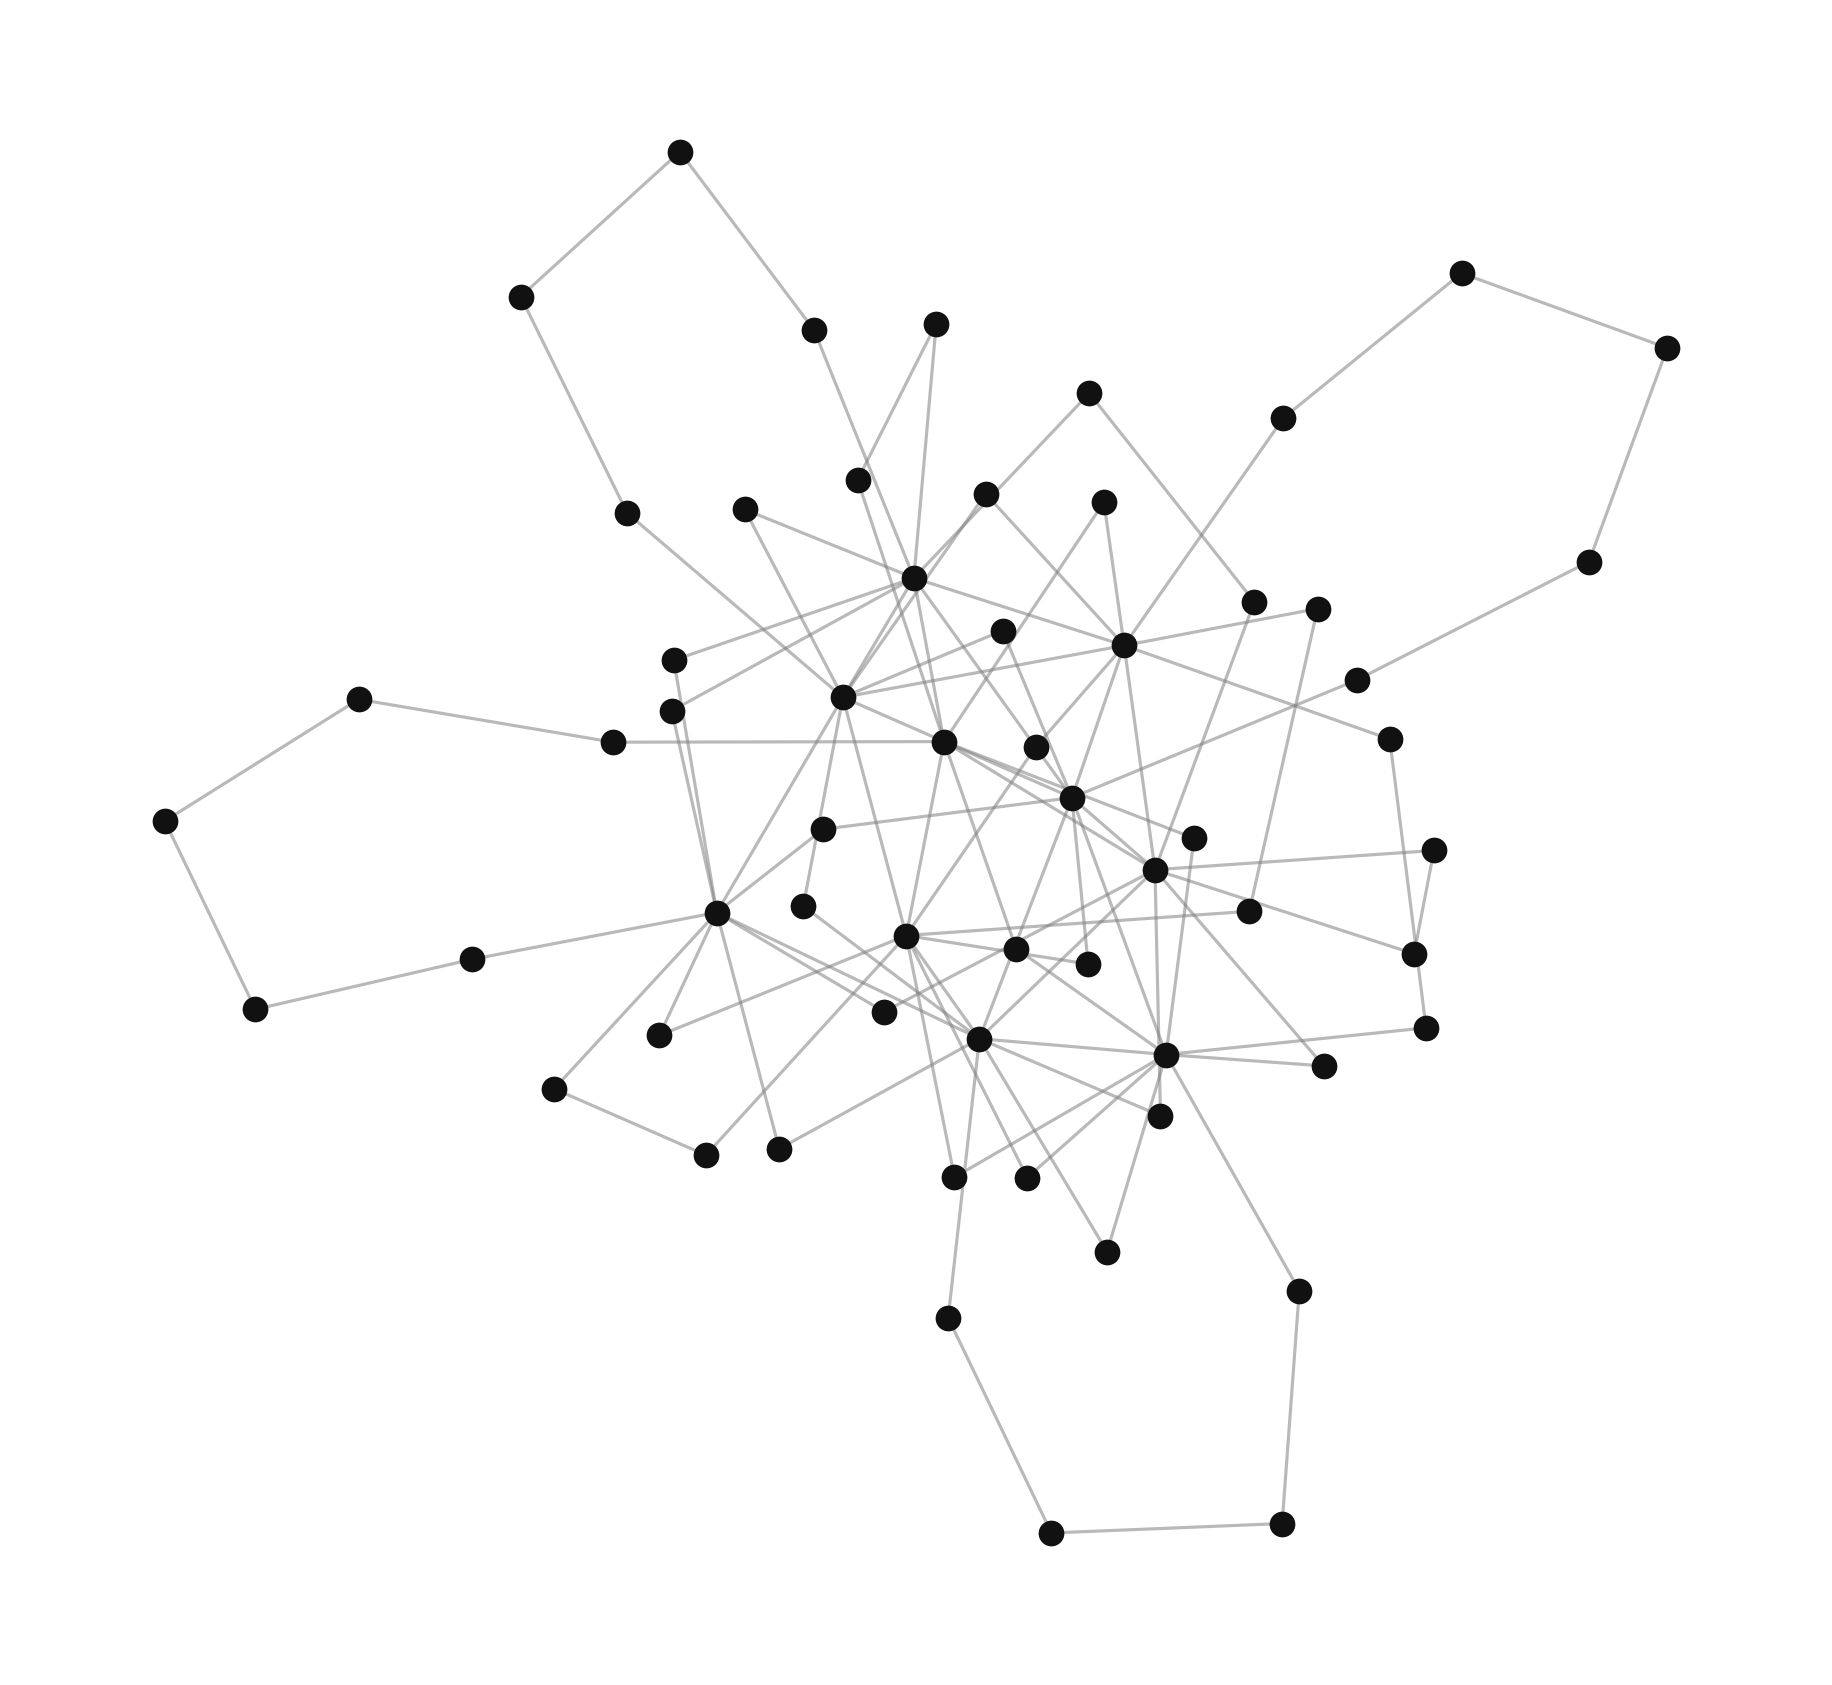
\includegraphics[width=0.62\textwidth]{figures/graph_models/configuration_model.png}
    \caption{Illustrative simple-graph realization with a prescribed
    heterogeneous degree sequence, consisting of 10 nodes of degree 10 and
    50 nodes of degree 2. The example highlights the defining role of the
    degree sequence while introducing no explicit community structure.}
    \label{fig:configuration_model}
\end{figure}

\subsection{Expected-degree models}
\label{subsec:expected_degree_models}

Expected-degree models were connected to product-form graphons in Section~\ref{subsec:smooth_rank_graphons}. In the Chung--Lu formulation, each node \(i\) is assigned a non-negative weight \(w_i\), and a common parameterization is

\[
p_{ij}
=
\frac{w_iw_j}{\sum_{k=1}^{n}w_k},
\]

under conditions ensuring \(p_{ij}\leq1\) \cite{chung2002connected}. Edges are sampled independently according to these probabilities, introducing degree heterogeneity without requiring discrete communities.
\begin{figure}[H]
    \centering
    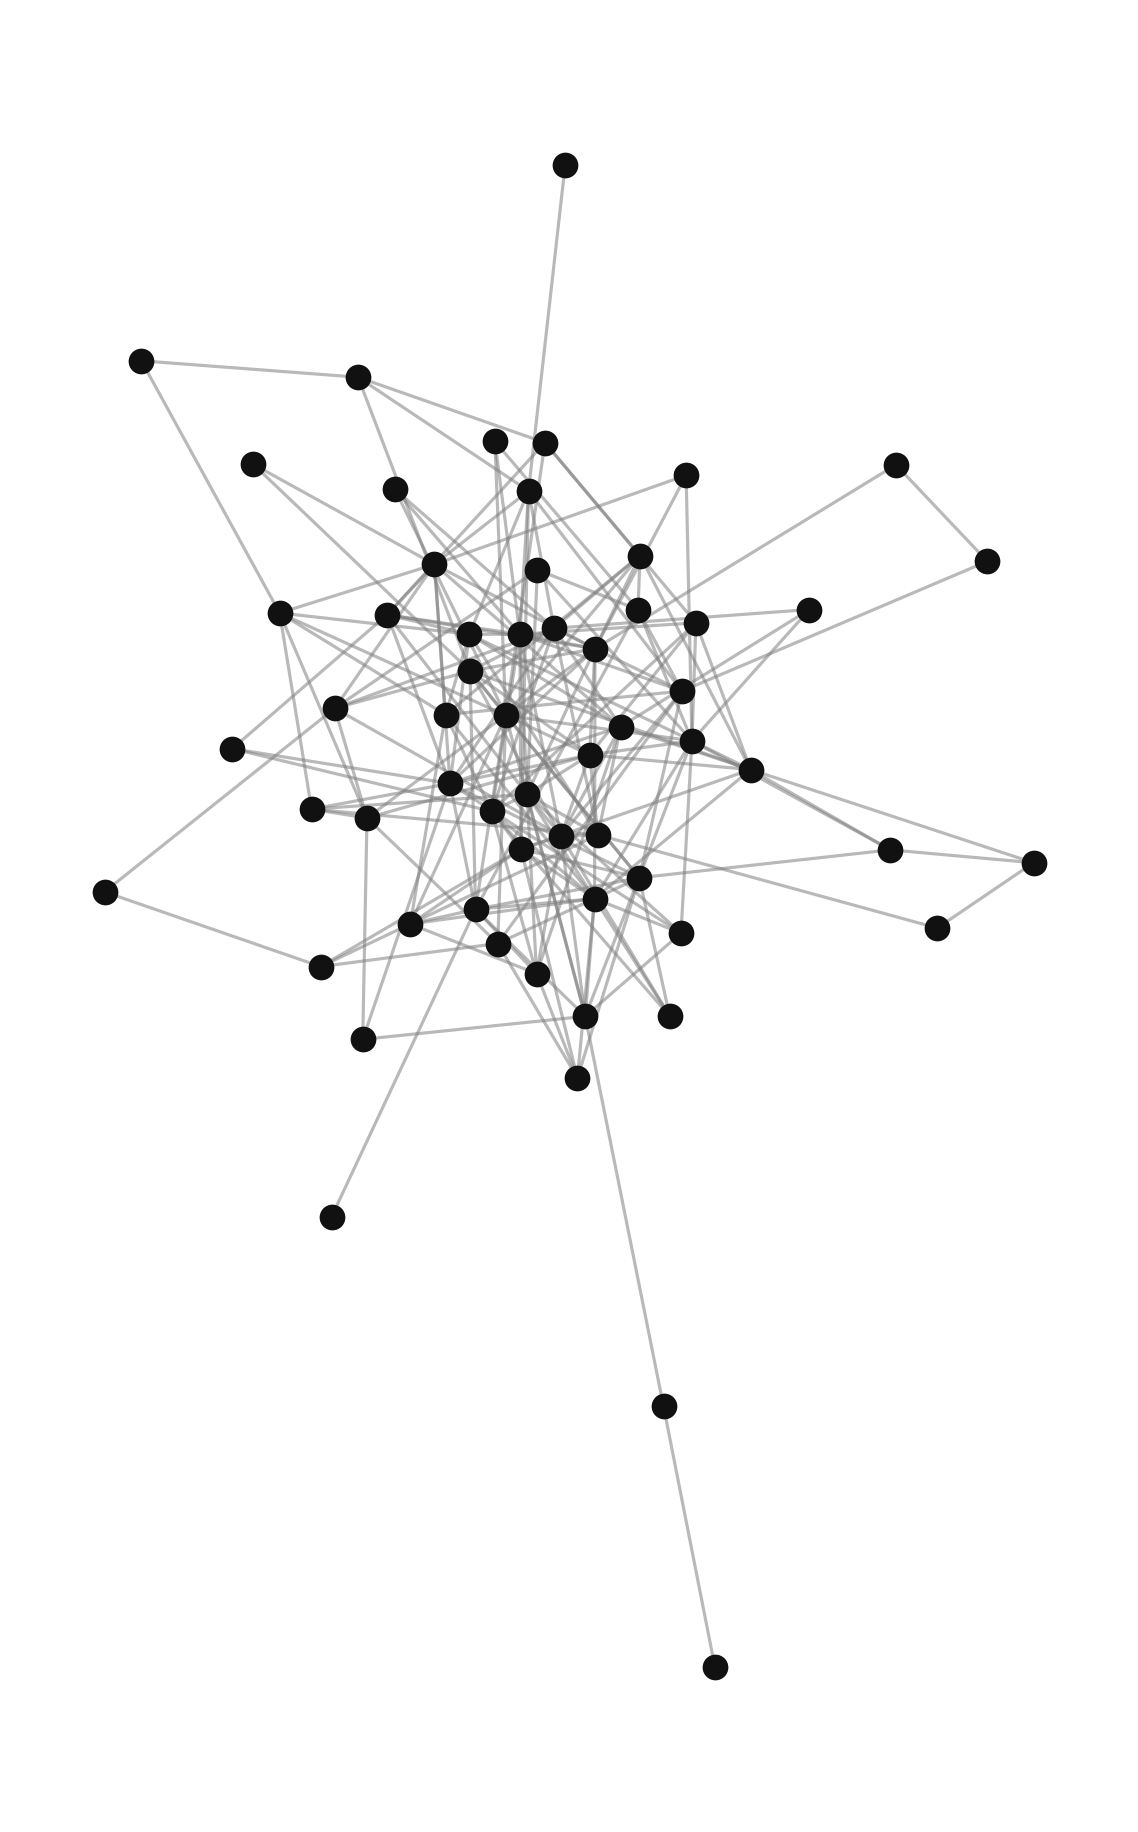
\includegraphics[width=0.62\textwidth]{figures/graph_models/expected_degree.png}
    \caption{Illustrative realization of an expected-degree random graph with
    $n=60$ and node-specific expected-degree parameters ranging from 1 to 12.
    Unlike a fixed-degree construction, these parameters determine edge
    probabilities rather than exact realized degrees, producing gradual
    heterogeneity in node connectivity.}
    \label{fig:expected_degree}
\end{figure}

\subsection{Barab\'asi--Albert model}
\label{subsec:barabasi_albert}

The Barab\'asi--Albert model generates a growing graph through preferential attachment \cite{barabasi1999emergence}. Each newly introduced node creates \(m\) edges to existing nodes, and node \(i\) is selected with probability

\[
\Pi(i)
=
\frac{d_i}{\sum_j d_j},
\]

where \(d_i\) is its current degree. This reinforcement mechanism favors already well-connected nodes and produces heterogeneous, hub-dominated degree distributions.
\begin{figure}[H]
    \centering
    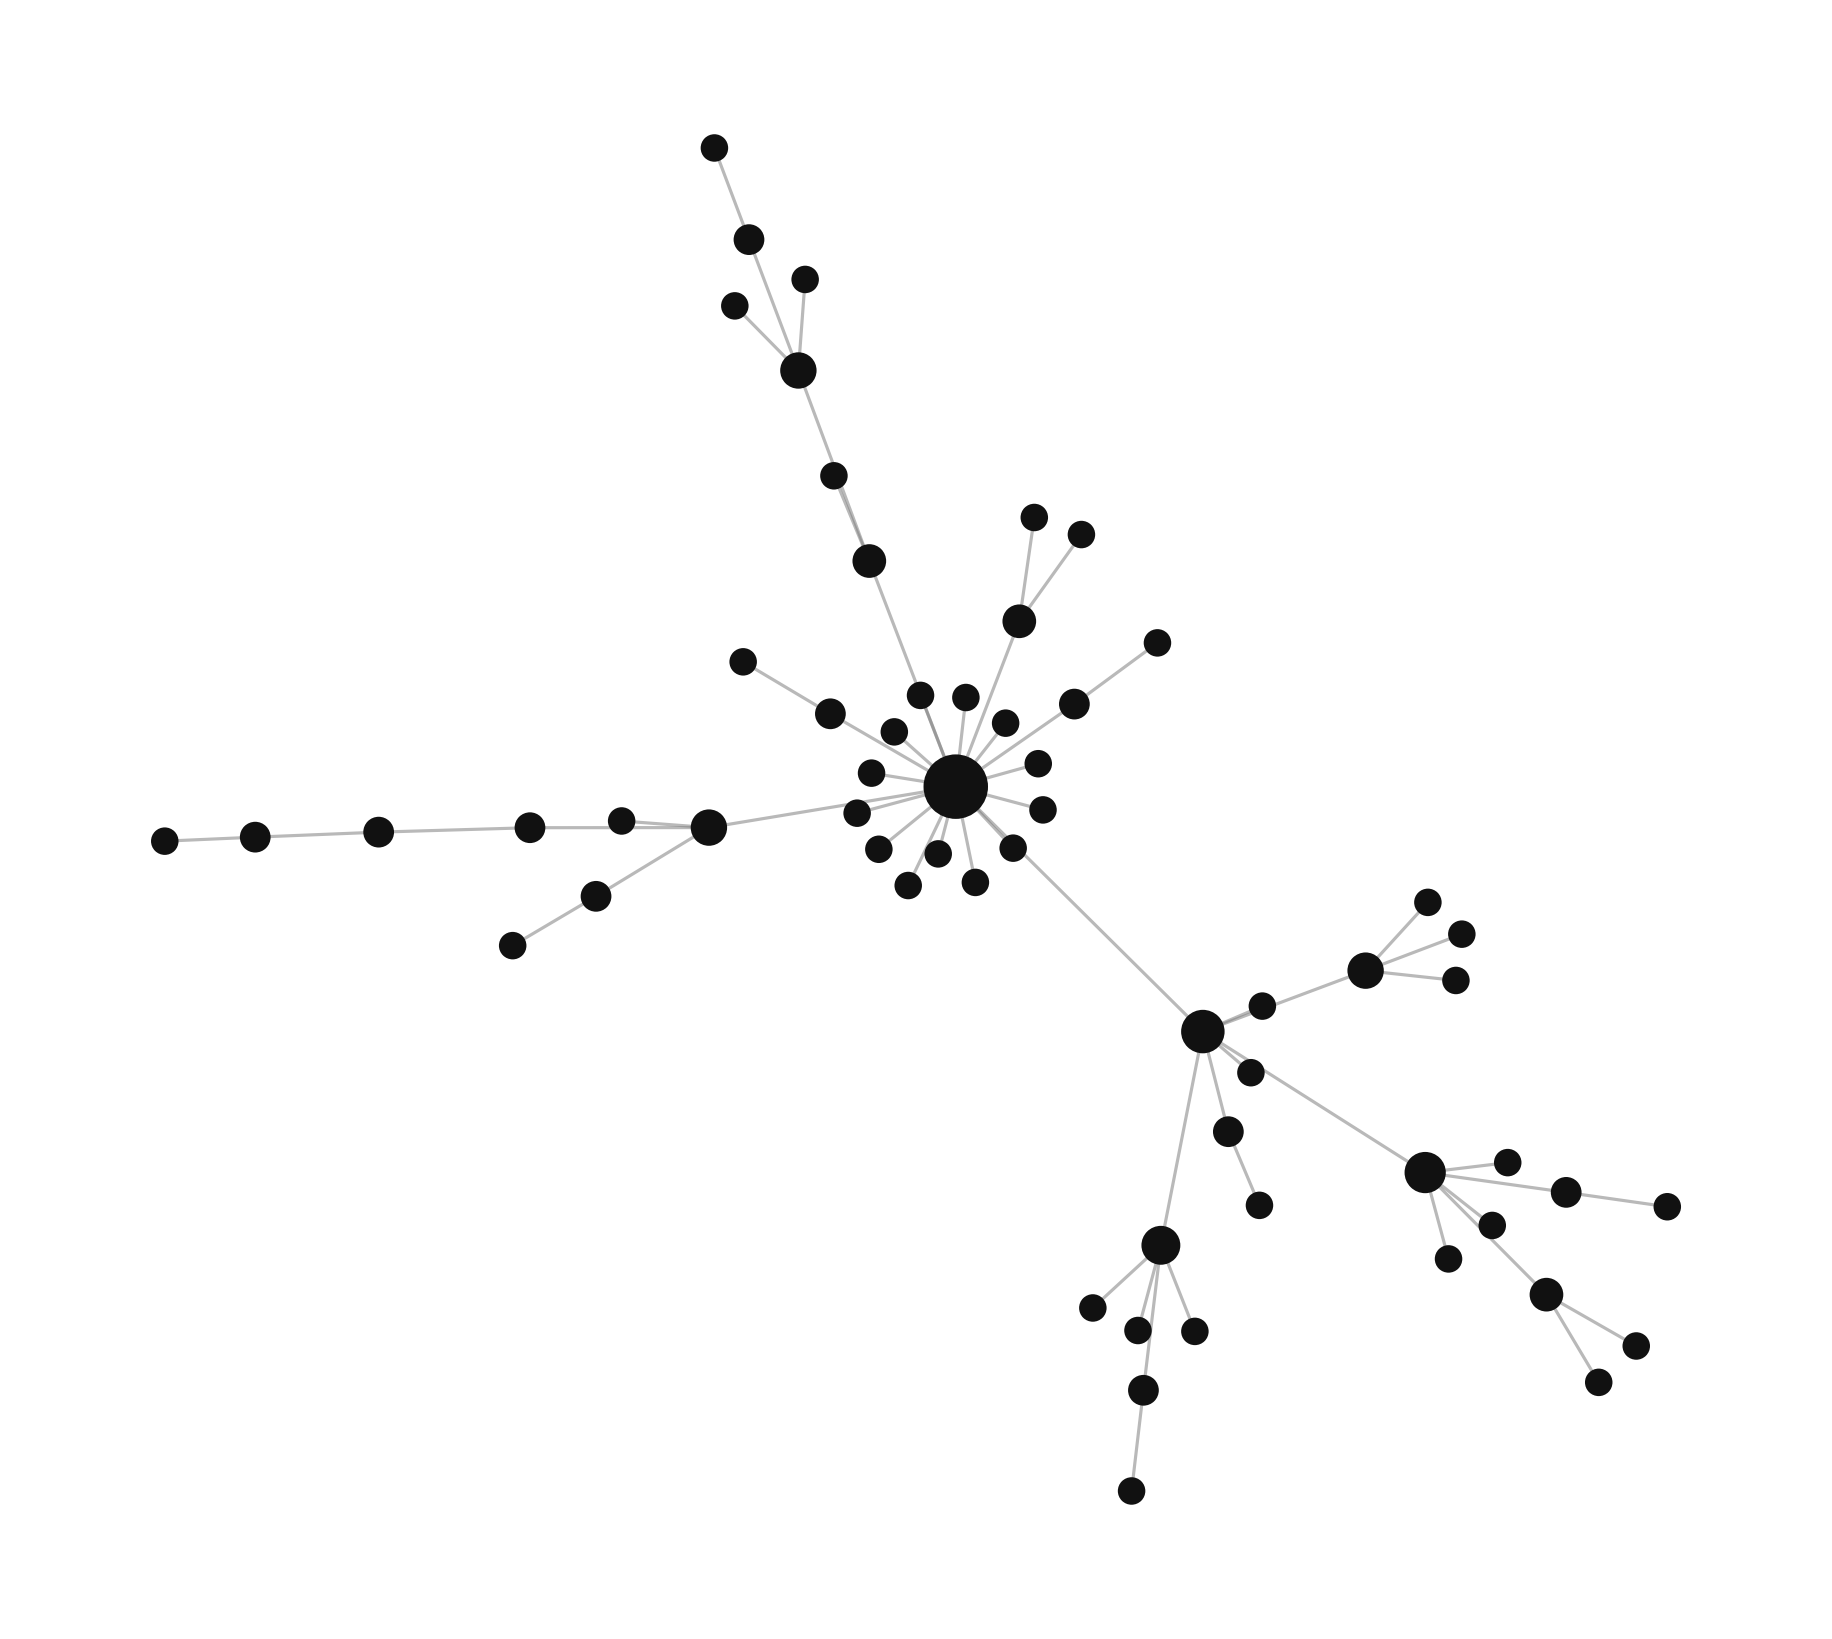
\includegraphics[width=0.3\textwidth]{figures/graph_models/barabasi_albert.png}
    \caption{Illustrative realization of a Barabási--Albert graph with
    $n=60$ and attachment parameter $m=1$. Nodes are added sequentially and
    preferentially attach to already well-connected nodes, producing a sparse,
    hub-dominated network with heterogeneous degrees. Node size is proportional
    to the realized degree to make the hub structure visually explicit.}
    \label{fig:barabasi_albert}
\end{figure}

\subsection{Watts--Strogatz model}
\label{subsec:watts_strogatz}

The Watts--Strogatz model starts from a regular ring lattice in which each node is connected to a fixed number \(k\) of nearby nodes and rewires edges with probability \(\beta\in[0,1]\) \cite{watts1998collective}. Intermediate values of \(\beta\) can combine relatively high local clustering with short characteristic path lengths.
\begin{figure}[H]
    \centering
    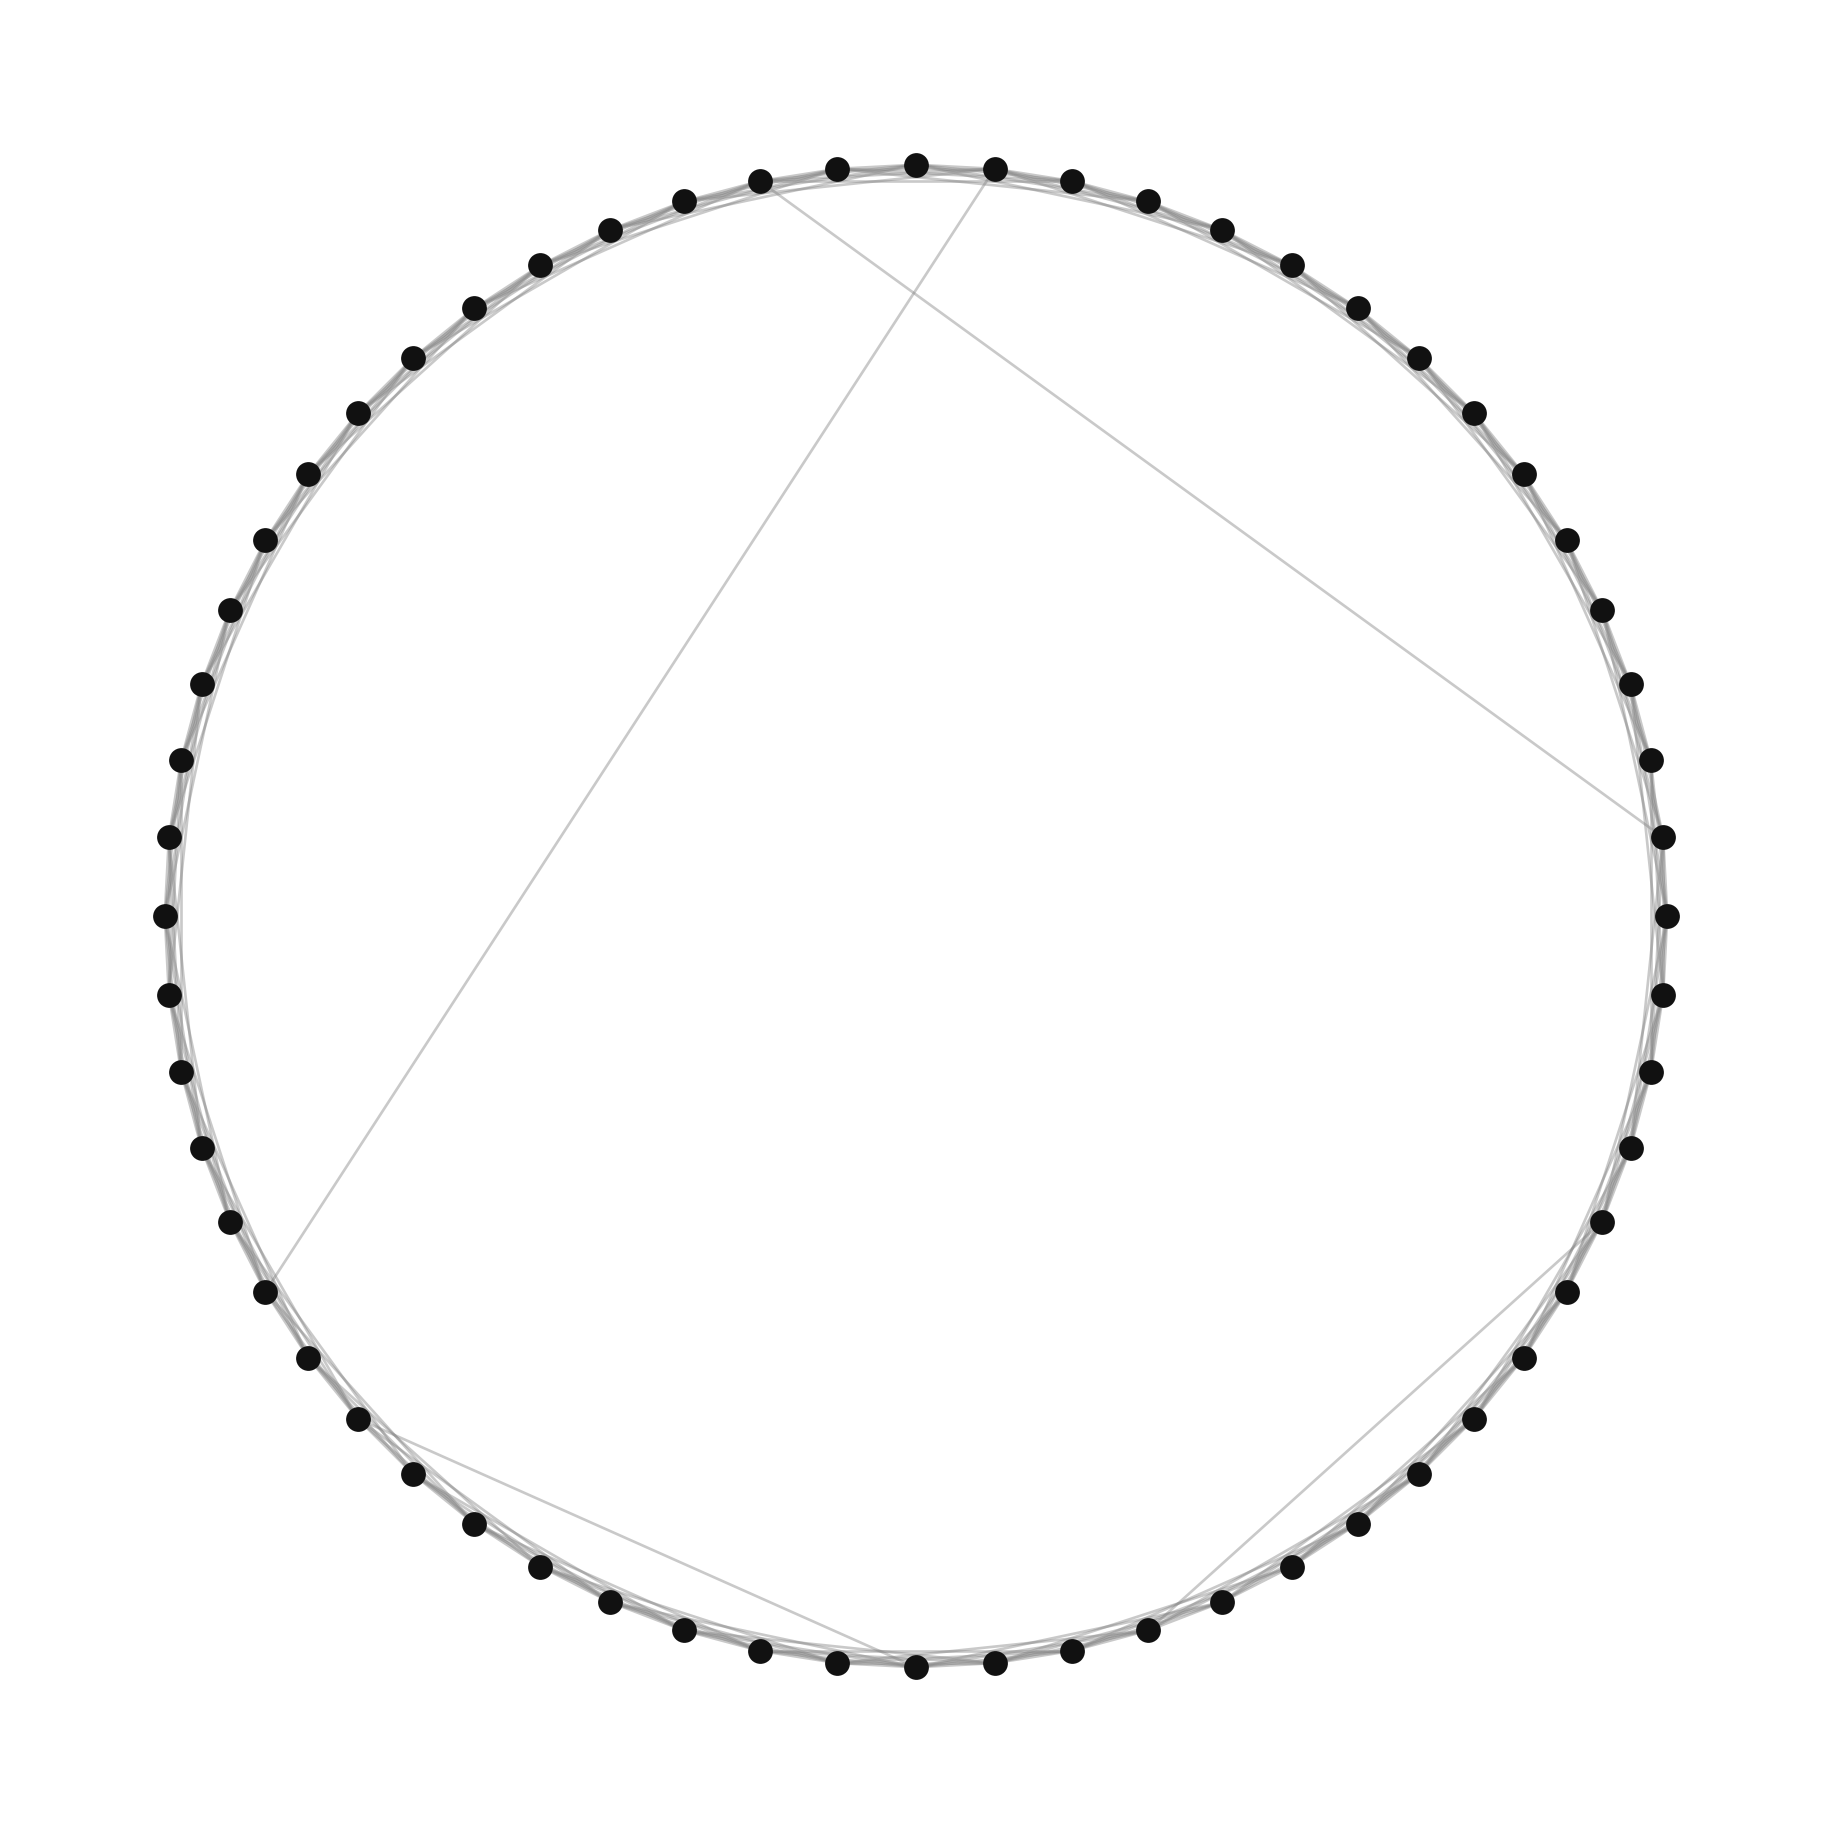
\includegraphics[width=0.3\textwidth]{figures/graph_models/watts_strogatz.png}
    \caption{Illustrative realization of a Watts--Strogatz small-world graph
    with $n=60$, neighborhood size $k=8$, and rewiring probability $p=0.03$.
    The circular layout exposes the underlying locally connected ring lattice,
    while the few long-range edges crossing the circle illustrate the
    shortcuts introduced by random rewiring.}
    \label{fig:watts_strogatz}
\end{figure}

\section{Graphon Estimation}
\label{sec:rw_graphon_estimation}

The general graphon-estimation problem, including latent positions, arbitrary node ordering, and non-identifiability, was introduced in Section~\ref{sec:graphon_estimation}. The methods reviewed here differ primarily in how they address these difficulties and represent the estimated probability function.


\subsection{Structured, ordering-based, and smoothing estimators}
\label{subsec:rw_classical_graphon_estimators}

Airoldi, Costa, and Chan estimate graphons through stochastic-blockmodel approximations, yielding piecewise-constant representations over finite partitions of the graphon domain \cite{airoldi2013stochastic}.

Gao, Lu, and Zhou characterize minimax rates under different structural and smoothness assumptions \cite{gao2015rate}. A minimax rate describes the best worst-case convergence rate attainable over a prescribed class of graphons. Their analysis highlights the contribution of latent node-ordering uncertainty to estimation difficulty.

Chan and Airoldi address node organization explicitly through their Sorting-and-Smoothing estimator \cite{chan2014consistent}. Nodes are sorted according to empirical degree, the reordered adjacency matrix is aggregated into a histogram, and total-variation regularization penalizes abrupt local variations while allowing discontinuities.

Neighbourhood smoothing instead estimates edge probabilities by averaging across nodes with similar observed connectivity profiles \cite{zhang2017estimating}.

Xu studies Universal Singular Value Thresholding (USVT), which performs a singular-value decomposition and discards components whose singular values fall below a threshold before reconstructing the probability matrix \cite{xu2018rates}.

These methods therefore use block structure, degree-based ordering, neighbourhood similarity, or spectral low-rank structure as their principal regularization mechanisms.


\subsection{Alignment-aware and neural graphon representations}
\label{subsec:rw_neural_graphon_estimators}

When observed graphs have different sizes and no known node correspondence, alignment becomes part of the estimation problem. Xu et al. formulate graphon estimation through structured Gromov--Wasserstein barycenters \cite{xu2021structured}. A transport coupling defines a soft correspondence between two structures, while the Gromov--Wasserstein discrepancy compares their internal relational structure rather than requiring direct node correspondence. A barycenter then provides a common representation minimizing aggregate discrepancy from the observed graphs.

IGNR uses the implicit neural representations introduced in Section~\ref{subsec:implicit_representations} to replace a fixed-resolution graphon by a continuous coordinate-based neural function \cite{xia2023implicit}. Gromov--Wasserstein comparison remains part of the fitting procedure, allowing unaligned and differently sized graphs to contribute to a common estimate.

SIGL, proposed by Azizpour, Zilberstein, and Segarra, separates node organization and graphon regression more explicitly \cite{azizpour2025scalable}. A Graph Neural Network (GNN) computes node representations by aggregating and transforming information from graph neighbourhoods in a manner that can be made consistent with node permutations.

Consider

\[
\mathcal{D}
=
\{A_t\}_{t=1}^{M},
\]

where \(M\) is the number of observed graphs and

\[
A_t\in\{0,1\}^{n_t\times n_t}
\]

is the adjacency matrix of graph \(t\), containing \(n_t\) nodes.

SIGL first uses a GNN \(g_{\phi_1}\), parameterized by \(\phi_1\), to infer scalar node coordinates:

\[
\hat{\boldsymbol{\eta}}_t
=
g_{\phi_1}(A_t,X_t),
\]

where

\[
\hat{\boldsymbol{\eta}}_t
=
(\hat{\eta}_{t,1},\ldots,\hat{\eta}_{t,n_t})
\]

contains the predicted coordinates and \(X_t\) denotes the node features supplied to the network. In the original formulation, these are randomly generated Gaussian features rather than semantic node attributes.

An auxiliary implicit function \(h_{\phi_2}\), with parameters \(\phi_2\), maps pairs of predicted coordinates to estimated adjacency values. The two components are jointly fitted through

\[
\mathcal{L}(\phi)
=
\sum_{t=1}^{M}
\frac{1}{n_t^2}
\sum_{i=1}^{n_t}
\sum_{j=1}^{n_t}
\left[
A_t(i,j)
-
h_{\phi_2}
\left(
\hat{\eta}_{t,i},
\hat{\eta}_{t,j}
\right)
\right]^2,
\]

where

\[
\phi=(\phi_1,\phi_2).
\]

The predicted coordinates are then used to reorder each adjacency matrix. Let \(\hat{A}_t\) denote the reordered matrix. For a pooling-window side length \(h\),

\[
\hat{H}_t
\in
\mathbb{R}^{k_t\times k_t},
\qquad
k_t
=
\left\lfloor
\frac{n_t}{h}
\right\rfloor,
\]

with entries

\[
\hat{H}_t(i,j)
=
\frac{1}{h^2}
\sum_{s_1=1}^{h}
\sum_{s_2=1}^{h}
\hat{A}_t
\left(
(i-1)h+s_1,
(j-1)h+s_2
\right).
\]

The pooled values are interpreted as coordinate--value observations of a common graphon:

\[
\mathcal{C}
=
\left\{
\left(
\frac{i}{k_t},
\frac{j}{k_t},
\hat{H}_t(i,j)
\right)
:
t=1,\ldots,M,\;
i,j=1,\ldots,k_t
\right\}.
\]

A second implicit neural representation

\[
f_\theta:[0,1]^2\rightarrow[0,1]
\]

is fitted through

\[
\theta^\star
=
\arg\min_{\theta}
\sum_{(u,v,y)\in\mathcal{C}}
\left[
f_\theta(u,v)-y
\right]^2.
\]

Here, \(u\) and \(v\) are normalized graphon coordinates and \(y\) is the corresponding pooled adjacency value.

As discussed in Section~\ref{subsec:numerical_graphon_representation}, the resulting continuous function can subsequently be evaluated at a chosen finite resolution. The principal distinction from IGNR is the treatment of alignment: IGNR retains Gromov--Wasserstein comparison during fitting, whereas SIGL first learns a node ordering and then reduces the final graphon-estimation stage to coordinate-based regression \cite{xia2023implicit,azizpour2025scalable}.


\section{Deep Graph Generative Models}
\label{sec:rw_graph_generation}

The graph-generation problem and the role of arbitrary node ordering were introduced in Section~\ref{sec:graph_generation_problem}. Neural graph generators differ in the probabilistic representation through which they approximate the target graph distribution.


\subsection{Autoregressive and sequential generation}
\label{subsec:rw_autoregressive_generation}

GraphRNN factorizes graph generation autoregressively \cite{you2018graphrnn}. Given a node ordering \(\pi\), let

\[
S^\pi
=
\left(
S^\pi_1,\ldots,S^\pi_n
\right)
\]

denote the resulting sequence, where \(S^\pi_i\) describes the edges connecting the \(i\)-th node to previously generated nodes. Its probability is

\[
p(S^\pi)
=
\prod_{i=1}^{n}
p
\left(
S^\pi_i
\mid
S^\pi_{<i}
\right),
\]

where

\[
S^\pi_{<i}
=
(S^\pi_1,\ldots,S^\pi_{i-1}).
\]

A graph-level recurrent network summarizes the partial graph, while the full GraphRNN model uses an additional edge-level recurrent network to generate the individual edges associated with each new node.

To reduce the ordering ambiguity discussed in Section~\ref{subsec:arbitrary_node_ordering}, GraphRNN restricts generation to breadth-first-search (BFS) orderings, which traverse a graph level by level from a starting node \cite{you2018graphrnn}.

GRAN instead generates blocks of nodes and edges autoregressively \cite{liao2019efficient}. Its attention-based GNN assigns learned weights to node interactions, while a mixture of Bernoulli distributions introduces dependencies among edge decisions within the same block. GRAN further marginalizes over a family of canonical node orderings.


\subsection{Latent and indirect graph representations}
\label{subsec:rw_latent_graph_generation}

A Variational Autoencoder (VAE) introduces a latent variable \(z\) through an encoder

\[
q_\phi(z\mid G),
\]

a prior \(p(z)\), and a decoder

\[
p_\theta(G\mid z),
\]

with training balancing reconstruction against regularization of the approximate latent posterior toward the prior.

GraphVAE adapts this framework to graphs \cite{simonovsky2018graphvae}. It decodes the latent representation into a probabilistic fully connected graph up to a fixed maximum size and performs approximate graph matching before evaluating reconstruction, preventing the loss from depending directly on arbitrary target node labels.

NetGAN instead learns the distribution of biased random walks sampled from an observed network \cite{bojchevski2018netgan}. A generator produces synthetic walks while an adversarial critic attempts to distinguish them from observed ones using a Wasserstein GAN objective. After training, transition frequencies accumulated from generated walks are converted into an edge-weight matrix from which a graph is reconstructed.


\section{Diffusion-Based Graph Generation}
\label{sec:rw_diffusion}

Diffusion models define generation through a predefined forward process that progressively corrupts data and a learned reverse process that attempts to undo this corruption \cite{ho2020denoising}.

Let \(x_0\) denote a clean sample and \(x_1,\ldots,x_T\) its progressively corrupted states. A discrete-time Markov forward process factorizes as

\[
q(x_{1:T}\mid x_0)
=
\prod_{t=1}^{T}
q(x_t\mid x_{t-1}),
\]

while a reverse model parameterized by \(\theta\) is

\[
p_\theta(x_{0:T-1}\mid x_T)
=
\prod_{t=1}^{T}
p_\theta(x_{t-1}\mid x_t).
\]

Generation starts from the terminal noise distribution and repeatedly applies the learned reverse transitions. For graph generation, an important distinction concerns whether the corrupted state is continuous or categorical.


\subsection{Score-based generation in the graph domain}
\label{subsec:rw_score_graph_generation}

Score-based generative modeling learns the score of a probability distribution, namely the gradient of its log-density with respect to the current state.

Niu et al. apply this framework to continuously perturbed adjacency representations \cite{niu2020permutation}. Let \(A_t\) denote a noisy adjacency representation at noise level \(t\), and let \(p_t(A_t)\) denote its density. A neural network \(s_\theta\) approximates

\[
s_\theta(A_t,t)
\approx
\nabla_{A_t}
\log p_t(A_t).
\]

To satisfy the permutation requirement discussed in Section~\ref{subsec:arbitrary_node_ordering}, the network is permutation equivariant:

\[
s_\theta
\left(
P A_t P^\top,t
\right)
=
P\,
s_\theta(A_t,t)\,
P^\top,
\]

for any permutation matrix \(P\).

Training uses score matching, while generation uses annealed Langevin dynamics, a stochastic sampling procedure guided by the learned score as the noise level is progressively reduced.

Jo, Lee, and Hwang extend this framework to continuous time \cite{jo2022score}. A stochastic differential equation (SDE) has generic form

\[
dZ_t
=
f(Z_t,t)\,dt
+
g(Z_t,t)\,dB_t,
\]

where \(f\) is the drift, \(g\) controls the stochastic component, and \(B_t\) is Brownian motion. Jo et al. construct coupled SDEs for node features and adjacency variables and generate graphs through the corresponding reverse-time system.


\subsection{Discrete-state diffusion}
\label{subsec:rw_discrete_graph_diffusion}

Austin et al. introduce Discrete Denoising Diffusion Probabilistic Models (D3PMs), extending diffusion modeling to categorical state spaces \cite{austin2021structured}.

Let

\[
\mathbf{x}_t\in\{0,1\}^{K}
\]

denote the one-hot representation of a categorical variable with \(K\) states at diffusion step \(t\). A forward transition is parameterized by a row-stochastic matrix

\[
Q_t\in[0,1]^{K\times K},
\]

where \(Q_t(i,j)\) is the probability of transitioning from category \(i\) to category \(j\):

\[
q(\mathbf{x}_t\mid\mathbf{x}_{t-1})
=
\operatorname{Cat}
\left(
\mathbf{x}_t;
\mathbf{x}_{t-1}Q_t
\right).
\]

Define the cumulative transition matrix

\[
\overline{Q}_t
=
Q_1Q_2\cdots Q_t.
\]

The noisy state at time \(t\) can then be sampled directly from the clean state:

\[
q(\mathbf{x}_t\mid\mathbf{x}_0)
=
\operatorname{Cat}
\left(
\mathbf{x}_t;
\mathbf{x}_0\overline{Q}_t
\right).
\]

The posterior distribution of the previous state is analytically available:

\[
q
\left(
\mathbf{x}_{t-1}
\mid
\mathbf{x}_t,\mathbf{x}_0
\right)
=
\operatorname{Cat}
\left(
\mathbf{x}_{t-1};
\frac{
\mathbf{x}_t Q_t^\top
\odot
\mathbf{x}_0\overline{Q}_{t-1}
}{
\mathbf{x}_0\overline{Q}_t\mathbf{x}_t^\top
}
\right),
\]

where \(\odot\) denotes element-wise multiplication.

D3PM can parameterize the reverse process through clean-state predictions

\[
\widetilde{p}_\theta
\left(
\widetilde{\mathbf{x}}_0
\mid
\mathbf{x}_t
\right),
\]

which are combined with the known forward process to obtain

\[
p_\theta
\left(
\mathbf{x}_{t-1}
\mid
\mathbf{x}_t
\right)
\propto
\sum_{\widetilde{\mathbf{x}}_0}
q
\left(
\mathbf{x}_{t-1},
\mathbf{x}_t
\mid
\widetilde{\mathbf{x}}_0
\right)
\widetilde{p}_\theta
\left(
\widetilde{\mathbf{x}}_0
\mid
\mathbf{x}_t
\right).
\]

Austin et al. combine the variational diffusion objective with an auxiliary clean-state prediction loss:

\[
\mathcal{L}_{\lambda}
=
\mathcal{L}_{\mathrm{vb}}
+
\lambda
\,
\mathbb{E}
\left[
-\log
\widetilde{p}_\theta
\left(
\mathbf{x}_0
\mid
\mathbf{x}_t
\right)
\right].
\]

Here, \(\mathcal{L}_{\mathrm{vb}}\) is the variational upper bound on the negative log-likelihood, equivalently the negative evidence lower bound used as a minimization objective, and \(\lambda\geq0\) controls the auxiliary clean-state prediction term.

The transition matrices \(Q_t\) are an important modeling choice. D3PM considers uniform corruption, category-aware transitions, and absorbing-state corruption, in which the forward process eventually enters a designated state from which it cannot leave \cite{austin2021structured}.


\subsection{Direct discrete graph diffusion}
\label{subsec:rw_direct_graph_diffusion}

DiGress adapts discrete categorical diffusion directly to graph-valued data \cite{vignac2023digress}. A graph

\[
G=(X,E)
\]

with \(n\) nodes is represented by a node-category matrix

\[
X\in\{0,1\}^{n\times a}
\]

and an edge-category tensor

\[
E\in\{0,1\}^{n\times n\times b},
\]

where \(a\) and \(b\) are the numbers of possible node and edge categories. The absence of an edge is itself represented as an edge category.

Let

\[
G^t=(X^t,E^t)
\]

denote the corrupted graph at diffusion step \(t\). Separate transition matrices

\[
Q_X^t\in[0,1]^{a\times a},
\qquad
Q_E^t\in[0,1]^{b\times b}
\]

control node and edge corruption, with cumulative products

\[
\overline{Q}_X^t
=
Q_X^1Q_X^2\cdots Q_X^t,
\qquad
\overline{Q}_E^t
=
Q_E^1Q_E^2\cdots Q_E^t.
\]

Using the compact notation adopted in DiGress,

\[
q(G^t\mid G)
=
\left(
X\overline{Q}_X^t,
E\overline{Q}_E^t
\right),
\]

where the two terms parameterize the categorical marginal distributions of the node and edge states. Conditional on the clean graph, corruption is applied independently to the categorical variables while respecting edge symmetry.

The denoising network is a permutation-equivariant graph transformer that jointly updates node, edge, and graph-level representations through attention. Let

\[
\hat{p}_i^X
\]

and

\[
\hat{p}_{ij}^E
\]

denote the predicted clean-state distributions for node \(i\) and edge relation \((i,j)\), respectively. Training minimizes

\[
\mathcal{L}_{\mathrm{DiGress}}
=
\sum_{i=1}^{n}
\operatorname{CE}
\left(
x_i,\hat{p}_i^X
\right)
+
\lambda
\sum_{i,j}
\operatorname{CE}
\left(
e_{ij},\hat{p}_{ij}^E
\right),
\]

where \(\operatorname{CE}\) denotes categorical cross-entropy and \(\lambda\) controls the relative contribution of edge prediction.

During reverse sampling, the predicted clean-state distributions are combined with the analytical posterior induced by the forward transitions to construct

\[
p_\theta
\left(
G^{t-1}\mid G^t
\right).
\]

DiGress also considers transition models whose limiting distributions reproduce empirical node and edge marginals rather than necessarily converging to uniform noise. Structural and spectral quantities extracted from the noisy graph are additionally supplied as auxiliary features \cite{vignac2023digress}.

EDGE develops a discrete diffusion process motivated by sparse-graph scalability \cite{chen2023efficient}. Its forward process progressively removes edges toward the empty graph, while the reverse process restricts edge prediction to selected node subsets and explicitly models degree information.

DISCO instead formulates graph generation as a discrete-state continuous-time process \cite{xu2024discrete}. Node and edge states remain categorical, but transitions evolve in continuous time while preserving graph permutation symmetries.


\subsection{Diffusion in latent representations}
\label{subsec:rw_latent_diffusion}

Latent Graph Diffusion maps graph structure and attributes into a learned latent representation, performs diffusion in that space, and decodes generated latent states back into graphs \cite{zhou2024latent}. Unlike direct models such as DiGress, diffusion therefore acts on an encoded graph representation rather than explicit node and edge variables.


\section{Graphon-Mediated Graph Generation}
\label{sec:rw_graphon_generation}

The distinction between a mathematical graphon, a finite numerical representation, and a sampled binary graph was established in Sections~\ref{subsec:numerical_graphon_representation} and~\ref{subsec:graphon_sampling}. Graphon-mediated generators use the probability representation itself as part of the learned generative mechanism.


\subsection{Neural graphons as generative representations}
\label{subsec:rw_neural_graphon_generation}

Because an implicit graphon can be evaluated at a chosen finite resolution, as described in Section~\ref{subsec:implicit_representations}, IGNR can use its learned continuous function as a probability representation for subsequent graph sampling \cite{xia2023implicit}.

Xu et al. develop a graphon autoencoder in \emph{Learning Graphon Autoencoders for Generative Graph Modeling} \cite{xu2021graphonautoencoder}. Its encoder aggregates Chebyshev graphon filters, which combine structural information across multiple effective neighbourhood scales, into a low-dimensional latent representation. A linear graphon-factorization decoder then reconstructs graphon-valued outputs.

Training minimizes a Wasserstein discrepancy between model and data distributions, using the Kullback--Leibler divergence between graph distributions conditioned on different graphons as the transport cost. The reconstructed object is therefore a graph-generating probability representation rather than a single binary graph.


\subsection{Diffusion from a graphon perspective}
\label{subsec:rw_graphon_diffusion}

DiPhon provides a recent connection between graphons and diffusion-based graph generation \cite{rozada2026diphon}. In the dense-graph setting, it defines stochastic dynamics directly on graphon values through a Jacobi stochastic differential equation,

\[
dX_t
=
\kappa(\mu-X_t)\,dt
+
\sigma
\sqrt{X_t(1-X_t)}
\,dB_t,
\]

where \(X_t\in[0,1]\), \(\kappa\) controls mean reversion, \(\mu\in[0,1]\) is the mean-reversion level, \(\sigma\) controls stochastic variability, and \(B_t\) is Brownian motion. Under suitable parameter conditions, these dynamics remain compatible with probability-valued states in \([0,1]\).

DiPhon constructs a corresponding finite-graph process and generates through reverse-time dynamics depending on the marginal score. It establishes exact agreement of the first moment between the relevant finite and graphon-induced processes and an approximation result for the second moment \cite{rozada2026diphon}.

As a 2026 preprint, DiPhon represents a recent development; its relevance here is the definition of diffusion dynamics directly from a graphon representation rather than from a finite adjacency tensor.


\section{Evaluation of Graph Generative Models}
\label{sec:rw_evaluation}

The need for distributional evaluation was introduced in Section~\ref{subsec:structural_fidelity}. Degree distributions, clustering coefficients, and normalized-Laplacian spectra were defined in Sections~\ref{subsec:degree_density}, \ref{subsec:clustering_coefficient}, and~\ref{subsec:laplacian_spectrum}. The literature reviewed here concerns how such representations are compared and the limitations of the resulting evaluation procedures.


\subsection{Structural statistics and distributional comparison}
\label{subsec:rw_structural_evaluation}

GraphRNN helped establish an evaluation protocol in which distributions of graph statistics are compared between generated and reference graph sets using Maximum Mean Discrepancy (MMD) \cite{you2018graphrnn}. Additional statistics may include motifs, that is, small recurring subgraph patterns.

Let

\[
\phi(G)
\]

denote a descriptor mapping a graph \(G\) to a numerical representation. Suppose that \(m\) reference graphs and \(n\) generated graphs produce descriptor samples

\[
\{x_i\}_{i=1}^{m}
\qquad\text{and}\qquad
\{y_j\}_{j=1}^{n},
\]

respectively.

MMD compares the corresponding distributions through a positive-definite kernel \(k\) \cite{gretton2012kernel}. A common biased empirical estimator of squared MMD is

\[
\widehat{\operatorname{MMD}}_{\mathrm{b}}^2
=
\frac{1}{m^2}
\sum_{i=1}^{m}
\sum_{i'=1}^{m}
k(x_i,x_{i'})
+
\frac{1}{n^2}
\sum_{j=1}^{n}
\sum_{j'=1}^{n}
k(y_j,y_{j'})
-
\frac{2}{mn}
\sum_{i=1}^{m}
\sum_{j=1}^{n}
k(x_i,y_j).
\]

It is biased because the within-sample sums include diagonal terms such as \(k(x_i,x_i)\) and \(k(y_j,y_j)\).

The discrepancy depends on both the descriptor \(\phi\) and the kernel \(k\), and kernel hyperparameters may also influence the result. O'Bray et al. show that graph-generative evaluation can be sensitive to descriptor construction, histogram processing, kernel choice, and kernel hyperparameters \cite{obray2022evaluation}. A low MMD value should therefore be interpreted as similarity under the chosen descriptor and evaluation procedure rather than equality of complete graph distributions.


\subsection{Learned and representation-based evaluation}
\label{subsec:rw_learned_evaluation}

The limitations of handcrafted statistics have motivated evaluation in learned representation spaces. A graph embedding is a fixed-dimensional vector summarizing structural or attribute information from a graph.

Thompson et al. investigate embeddings produced by Graph Neural Networks, including randomly initialized networks not trained for a specific downstream task \cite{thompson2022evaluation}. Generated and reference graphs are mapped into the resulting feature space, where their distributions can be compared.

Shirzad, Hassani, and Sutherland instead use representations learned through contrastive learning \cite{shirzad2022evaluating}. Contrastive objectives encourage representations of related graph views to be similar while separating unrelated samples.

Southern et al. explore alternatives based on graph curvature and topological filtrations \cite{southern2023curvature}. These descriptors capture structural information that may not be visible through conventional degree or clustering statistics.


\section{Summary and Methodological Positioning}
\label{sec:rw_summary}

The reviewed methods differ primarily in the representation on which estimation or generation is defined. Graphon estimation ranges from structured finite approximations to alignment-aware and continuous neural representations, with SIGL specifically separating learned node organization from implicit graphon regression.

Graph generators operate instead on sequential graph constructions, latent representations, perturbed continuous states, categorical node--edge variables, or learned latent spaces. D3PM provides the categorical diffusion framework most directly relevant to discrete-state generation, while DiGress applies discrete diffusion directly to graph variables.

Graphon-mediated approaches place edge-probability representations inside the generative process, whereas graph-generation evaluation compares generated and reference distributions through selected structural descriptors or learned representations. Consequently, both generation and evaluation remain strongly dependent on the representation in which the problem is formulated.
